\documentclass{article}
\usepackage[paperwidth=2.72in, paperheight=4.9in, margin=0.1in]{geometry}
\pagestyle{empty}
\usepackage{tikz}
\usetikzlibrary{arrows.meta, fit, backgrounds}
\usepackage{xcolor}

% Colors
\definecolor{cInput}{HTML}{EDE8DC}  \definecolor{bInput}{HTML}{8B7355}
\definecolor{cChan}{HTML}{FDEBD0}   \definecolor{bChan}{HTML}{CA6F1E}
\definecolor{cProc}{HTML}{EAF3FB}   \definecolor{bProc}{HTML}{2980B9}
\definecolor{cMask}{HTML}{D5F5E3}   \definecolor{bMask}{HTML}{1A8048}
\definecolor{cAn}{HTML}{D6EEF8}     \definecolor{bAn}{HTML}{117A8B}
\definecolor{cOut}{HTML}{D4EDDA}    \definecolor{bOut}{HTML}{1D7A38}
\definecolor{bgSeg}{HTML}{F5F5FF}   \definecolor{bdSeg}{HTML}{AAAADD}
\definecolor{bgAn}{HTML}{F0F8FF}    \definecolor{bdAn}{HTML}{88CCEE}
\definecolor{bgOut}{HTML}{F0FFF0}   \definecolor{bdOut}{HTML}{88DD88}

\tikzset{
  box/.style={draw, rounded corners=1.5pt, align=center,
              minimum height=0.5cm, text width=1.05cm, inner sep=1.5pt, line width=0.4pt},
  inputbox/.style={box, fill=cInput, draw=bInput, font=\fontsize{6.5}{7}\selectfont},
  chanbox/.style={box, fill=cChan, draw=bChan, font=\fontsize{5.5}{6}\selectfont},
  procbox/.style={box, fill=cProc, draw=bProc, font=\fontsize{5.5}{6}\selectfont},
  maskbox/.style={box, fill=cMask, draw=bMask, font=\fontsize{5.5}{6}\selectfont},
  anbox/.style={box, fill=cAn, draw=bAn, font=\fontsize{5.5}{6}\selectfont, text width=1.2cm},
  outbox/.style={box, fill=cOut, draw=bOut, font=\fontsize{5.5}{6}\selectfont},
  arr/.style={-{Stealth[length=2pt,width=1.5pt]}, draw=gray!50, line width=0.4pt},
  seclbl/.style={font=\fontsize{5}{5.5}\selectfont\itshape, text=gray!60},
}

\newcommand{\sub}[1]{{\fontsize{4.5}{5}\selectfont #1}}

\begin{document}
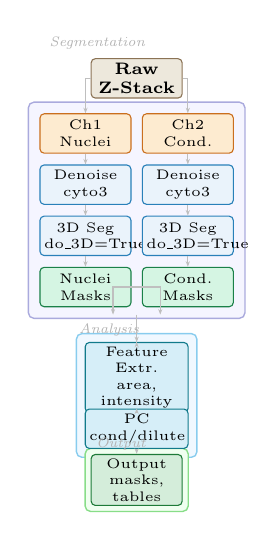
\begin{tikzpicture}

% Input
\node[inputbox] (raw) at (0, 4.3) {\textbf{Raw Z-Stack}};

% Section 1: Channel split
\node[chanbox] (ch1) at (-0.65, 3.6) {Ch1\\\sub{Nuclei}};
\node[chanbox] (ch2) at (0.65, 3.6) {Ch2\\\sub{Cond.}};
\draw[arr] (raw) -| (ch1);
\draw[arr] (raw) -| (ch2);

% Denoise
\node[procbox] (dn1) at (-0.65, 2.95) {Denoise\\\sub{cyto3}};
\node[procbox] (dn2) at (0.65, 2.95) {Denoise\\\sub{cyto3}};
\draw[arr] (ch1) -- (dn1);
\draw[arr] (ch2) -- (dn2);

% 3D Segment
\node[procbox] (seg1) at (-0.65, 2.3) {3D Seg\\\sub{do\_3D=True}};
\node[procbox] (seg2) at (0.65, 2.3) {3D Seg\\\sub{do\_3D=True}};
\draw[arr] (dn1) -- (seg1);
\draw[arr] (dn2) -- (seg2);

% Masks
\node[maskbox] (m1) at (-0.65, 1.65) {Nuclei\\\sub{Masks}};
\node[maskbox] (m2) at (0.65, 1.65) {Cond.\\\sub{Masks}};
\draw[arr] (seg1) -- (m1);
\draw[arr] (seg2) -- (m2);

% Merge to center
\draw[arr] (m1.east) -| (0.3, 1.3);
\draw[arr] (m2.west) -| (-0.3, 1.3);
\draw[arr] (0, 1.3) -- (0, 0.95);

% Feature extraction
\node[anbox] (fe) at (0, 0.5) {Feature Extr.\\\sub{area, intensity}};
\draw[arr] (0, 0.95) -- (fe);

% Partition coefficient
\node[anbox] (pc) at (0, -0.15) {PC\\\sub{cond/dilute}};
\draw[arr] (fe) -- (pc);

% Output
\node[outbox] (out) at (0, -0.8) {Output\\\sub{masks, tables}};
\draw[arr] (pc) -- (out);

% Section backgrounds
\begin{scope}[on background layer]
  \node[fill=bgSeg, draw=bdSeg, rounded corners=2pt, line width=0.5pt,
        fit=(ch1)(ch2)(dn1)(dn2)(seg1)(seg2)(m1)(m2),
        inner sep=4pt] (segbg) {};
  \node[fill=bgAn, draw=bdAn, rounded corners=2pt, line width=0.5pt,
        fit=(fe)(pc),
        inner sep=3pt] (anbg) {};
  \node[fill=bgOut, draw=bdOut, rounded corners=2pt, line width=0.5pt,
        fit=(out),
        inner sep=2pt] (outbg) {};
\end{scope}

% Section labels (outside and above the backgrounds)
\node[seclbl] at (-0.5, 4.75) {Segmentation};
\node[seclbl] at (-0.35, 1.1) {Analysis};
\node[seclbl] at (-0.2, -0.35) {Output};

\end{tikzpicture}
\end{document}
